% Source for docs/static/img/mapl-layouts.svg. Rebuild from the repository root:
%   pdflatex -output-directory=/tmp docs/scripts/mapl-layouts.tex
%   pdf2svg /tmp/mapl-layouts.pdf docs/static/img/mapl-layouts.svg
%   python3 docs/scripts/prepare_rollout_svgs.py
% Keep the stage boundaries in prepare_rollout_svgs.py in sync with the row positions.
% Shared preamble for the CoMLRL training-flow diagrams. Paste it verbatim at the
% top of every diagram so each .tex stays standalone.
\documentclass[tikz,border=3pt]{standalone}
\usepackage{amsmath,amssymb,bm}
\usetikzlibrary{arrows.meta,positioning,calc,fit}

% Only these paints have dark-theme mappings (assets/_diagram-theme.scss).
\colorlet{agentA}{red!80!black}     % agent 1: policy, prompts, responses, loss
\colorlet{agentB}{blue!80!black}    % agent 2
\colorlet{learned}{orange!80!black} % learned evaluators: critic, reward model
\colorlet{update}{green!50!black}   % gradients and parameter updates
% Joint or shared quantities are black. Gray = black with fill opacity.

\tikzset{
  >={Stealth[length=3.2pt,width=3pt]},
  box/.style={draw, line width=1pt, inner sep=2.5pt, minimum height=13pt},
  policy/.style={box, rounded corners=3pt, minimum width=30pt},
  flow/.style={->, line width=.8pt},
  note/.style={font=\scriptsize, align=left},
  label/.style={anchor=west, font=\footnotesize},
}


% Supported actor/comparator layouts: actor side (left), comparator side (right).
% Rows are animation stages; avoid \frac and \_ (their rules animate as edges).
% The split into role responses is drawn with curves, which fade in with their row.
\begin{document}
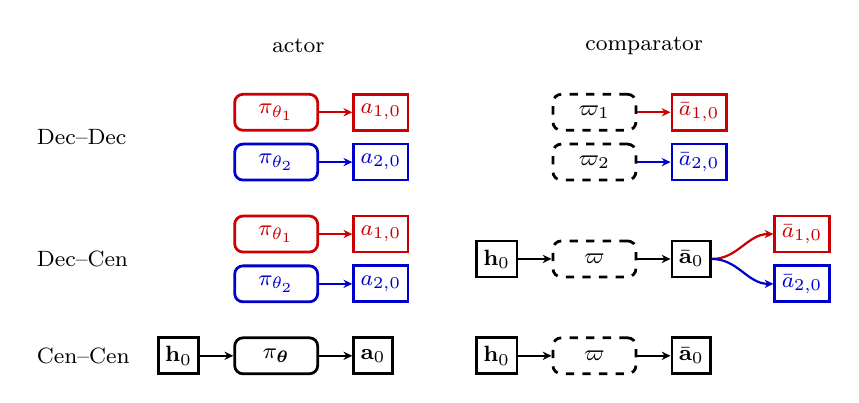
\begin{tikzpicture}[x=1pt, y=1pt, font=\footnotesize]
  \def\xp{90}   % actor policies
  \def\xq{205}   % comparators
  \def\xs{280}   % split role responses

  % Stage 0: the two sides of a comparison.
  \node at (\xp+8,0) {actor};
  \node at (\xq+18,0) {comparator};

  % Stage 1: one actor and one comparator per role.
  \node[label] at (0,-33) {Dec--Dec};
  \foreach \i/\c/\y in {1/agentA/-24, 2/agentB/-42} {
    \node[policy, \c] (p\i) at (\xp,\y) {$\pi_{\theta_{\i}}$};
    \node[box, \c, right=12pt of p\i] (a\i) {$a_{\i,0}$};
    \node[policy, dashed] (q\i) at (\xq,\y) {$\varpi_{\i}$};
    \node[box, \c, right=12pt of q\i] (b\i) {$\bar a_{\i,0}$};
    \draw[flow, \c] (p\i) -- (a\i);
    \draw[flow, \c] (q\i) -- (b\i);
  }

  % Stage 2: actors per role; one comparator writes the joint response,
  % which is split into role responses.
  \node[label] at (0,-77) {Dec--Cen};
  \foreach \i/\c/\y in {1/agentA/-68, 2/agentB/-86} {
    \node[policy, \c] (p\i) at (\xp,\y) {$\pi_{\theta_{\i}}$};
    \node[box, \c, right=12pt of p\i] (a\i) {$a_{\i,0}$};
    \draw[flow, \c] (p\i) -- (a\i);
  }
  \node[policy, dashed] (q) at (\xq,-77) {$\varpi$};
  \node[box, left=12pt of q] (h) {$\mathbf{h}_0$};
  \node[box, right=12pt of q] (j) {$\bar{\mathbf{a}}_0$};
  \node[box, agentA] (b1) at (\xs,-68) {$\bar a_{1,0}$};
  \node[box, agentB] (b2) at (\xs,-86) {$\bar a_{2,0}$};
  \draw[flow] (h) -- (q);
  \draw[flow] (q) -- (j);
  \draw[flow, agentA] (j.east) to[out=0, in=180] (b1.west);
  \draw[flow, agentB] (j.east) to[out=0, in=180] (b2.west);

  % Stage 3: one actor and one comparator, each writing the joint response.
  \node[label] at (0,-112) {Cen--Cen};
  \node[policy] (p) at (\xp,-112) {$\pi_{\bm{\theta}}$};
  \node[box, left=12pt of p] (ha) {$\mathbf{h}_0$};
  \node[box, right=12pt of p] (a) {$\mathbf{a}_0$};
  \node[policy, dashed] (q) at (\xq,-112) {$\varpi$};
  \node[box, left=12pt of q] (hq) {$\mathbf{h}_0$};
  \node[box, right=12pt of q] (b) {$\bar{\mathbf{a}}_0$};
  \draw[flow] (ha) -- (p);
  \draw[flow] (p) -- (a);
  \draw[flow] (hq) -- (q);
  \draw[flow] (q) -- (b);
\end{tikzpicture}
\end{document}
